\documentclass[a4paper, 11pt]{article}
\usepackage[brazil]{babel}
\usepackage[utf8]{inputenc}
\usepackage{blindtext}
\usepackage[top=3cm, left=2.5cm, right=2cm, bottom=2cm]{geometry}
\usepackage{amsthm,amsfonts}
\usepackage{graphicx}
\graphicspath{ {./img/} }
\setlength\parindent{0pt}

\author{Frederico Queiroz}
\title{Conceitos e Definições}

\begin{document}
\maketitle

%\section{Definições}

\section{Software}
\begin{itemize}
	\item \textbf{Software}: Programa de computador + Documentação associada.
	\item Desafios de Produzir Software: Confiabilidade, Preço e Desempenho, Sistemas Críticos.
	\item O desenvolvimento informal de software não é mais suficiente. Técnincas e métodos são necessários.
	\item Dificuldades em se produzir software: Heterogeneidade, Confiabilidade, Prazo de entrega, Mudança contínua.
\end{itemize}

\section{Engenharia de Software}
\begin{itemize}
	\item \textbf{Engenharia de Software}: É uma disciplina de engenharia que se preocupa com todos os aspectos de produção de software.
	\item Foco no desenvolvimento de software de \textbf{alta qualidade} dentro de \textbf{custos adequados}. Atender necessidades do cliente.		
	
	\item Diferença entre Engenharia de Software e outras Engenharias:
	\begin{itemize}
		\item Software é desenvolvido, não fabricado.
		\item Software não se desgasta.
		\item Software é geralmente produzido para um cliente específico.
	\end{itemize}
	
	\item Pode ser organizada em camadas com foco em qualidade:
	\begin{figure}[h]
		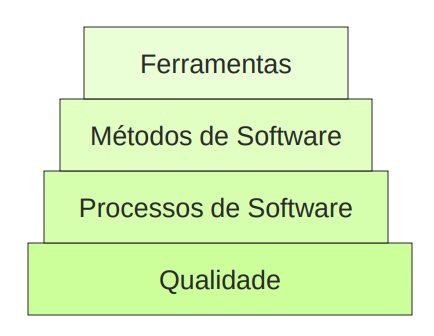
\includegraphics[width=6.5cm]{camadas_eng_soft}
		\centering
	\end{figure}

	\begin{itemize}
		\item \textbf{Qualidade}: Atributos de um bom software (Facilidade de manutenção, Confiança, Eficiência, Usabilidade, etc).
		
		\item \textbf{Processos de Software}: Atividades (e seus resultados) para o desenvolvimento de software (O que fazer?).
		\item Atividades principais:
		\begin{itemize}
			\item Especificação de requisitos
			\item Modelagem (Projeto de software)
			\item Implementação
			\item Verificação e Validação
			\item Evolução
		\end{itemize}
		
		\item \textbf{Métodos de Software}: Técnicas para desenvolvimento de software (Como fazer?). Métodos incluem Modelos, Notações, Regras, etc.
		
		\item \textbf{Ferramentas}: Fornecem apoio automatizado (ou semiautomatizado) para o processo e para os métodos (Ex.: ferramentas de modelagem do processo).
	\end{itemize}
\end{itemize}


\section{Processos de Software}
\begin{itemize}
	\item 5 atividades são comuns em \textbf{processos de desenvolvimento de software}:
	\begin{itemize}
		\item Especificação de requisitos
		\item Projeto de software (modelagem)
		\item Implementação
		\item Verificação e Validação
		\item Evolução
	\end{itemize}
\end{itemize}

\subsection{Especificação de requisitos}
\begin{itemize}
	\item \textbf{Requisitos} de um sistema são as descrições do que o sistema deve fazer, os serviços que oferece e as restrições a seu funcionamento.
	\item \textbf{Especificação de Requisitos} é o proceso de escrever os requisitos de \textbf{usuário} e de \textbf{sistema} em um documento de requisitos.
	\item Inclui quatro fases principais:
	\begin{figure}[h]
		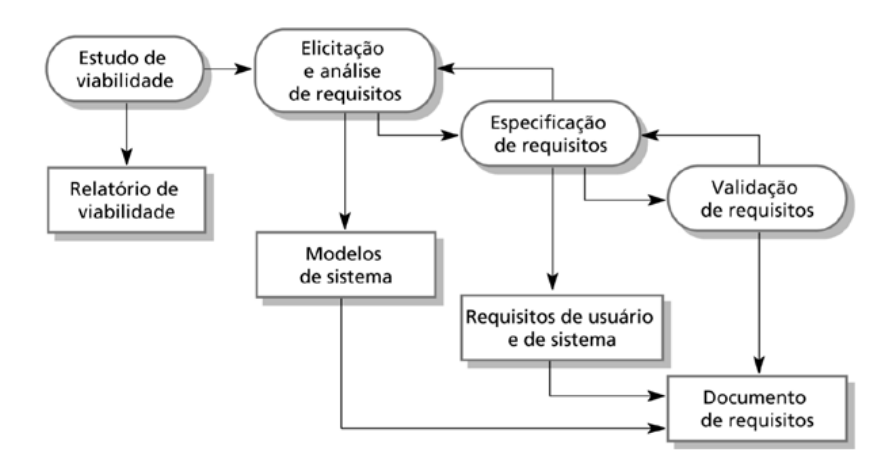
\includegraphics[width=12cm]{fases_espec_req}
		\centering
	\end{figure}
	\begin{itemize}
		\item \textbf{Estudo de viabilidade}: É feita uma estimativa da viabilidade. Considera-se restrições como, tecnologia atual, cronograma, orçamento, etc.
		\item \textbf{Elicitação (ou análise) de Requisitos}: Fase onde é derivado os requisitos do sistema. Usa-se várias técnicas baseadas em observação e entrevistas.
		\item \textbf{Especificação de Requisitos}: Etapa em que se traduz os requisitos obtidos em um documento. Os requisitos são catalogados e classificados.
		\item \textbf{Validação de Requisitos}: Avalia o documento de requisitos quanto ao realismo, consistência e completude. 
	\end{itemize}
\end{itemize}

\subsection{Projeto de Software (Modelagem)}
\begin{itemize}
	\item Dividido em duas etapas:
	\begin{itemize}
		\item \textbf{Projeto Preliminar}: define a estrutura modular do software, as interfaces e as estruturas de dados utilizadas. Modelo de Arquitetura.
		\item \textbf{Projeto Detalhado}: descreve detalhadamente cada módulo definido no projeto preliminar. Modelo de Projeto.
	\end{itemize}
\end{itemize}

\subsection{Implementação}
\begin{itemize}
	\item A implementação segue as definições da fase anterior (Projeto).
	\item Transcreve as decisões de projeto arquitetural e detalhado para uma linguagem de programação.
\end{itemize}

\subsection{Verificação e Validação}
\begin{itemize}
	\item Tem por objetivo garantir que o sistema satisfaça os requisitos.
	\item \textbf{Verificação} consiste na realização de alguns \textbf{testes} para encontrar erros.
	\item Deve ser feita a validação com o cliente.
	\item \textbf{Tipos de Testes}:
	\begin{itemize}
		\item \textbf{Teste de Unidade (Unitário)}: Garantir que um componente isolado funciona.
		\item \textbf{Teste de Integração}: Garantir que dois ou mais componentes funcionam juntos.
		\item \textbf{Teste de Aceitação}: Garantir que o sistema faz o que o cliente deseja.
	\end{itemize}
\end{itemize}

\subsection{Manutenção e Evolução}


\begin{itemize}
	\item Template
\end{itemize}

\end{document}